%% abtex2-modelo-trabalho-academico.tex, v-1.9.7 laurocesar
%% Copyright 2012-2018 by abnTeX2 group at http://www.abntex.net.br/
%%
%% This work may be distributed and/or modified under the
%% conditions of the LaTeX Project Public License, either version 1.3
%% of this license or (at your option) any later version.
%% The latest version of this license is in
%%   http://www.latex-project.org/lppl.txt
%% and version 1.3 or later is part of all distributions of LaTeX
%% version 2005/12/01 or later.
%%
%% This work has the LPPL maintenance status `maintained'.
%%
%% The Current Maintainer of this work is the abnTeX2 team, led
%% by Lauro C\'{e}sar Araujo. Further information are available on
%% http://www.abntex.net.br/

% ------------------------------------------------------------------------
% abnTeX2: Modelo de Trabalho Academico (tese de doutorado, dissertacao de
% mestrado e trabalhos monograficos em geral) em conformidade com
% ABNT NBR 14724:2011: Informacao e documentacao - Trabalhos academicos -
% Apresentacao
% ------------------------------------------------------------------------

% --- comeca preambulo ---
\documentclass[
	% -- op\c{c}\~{o}es da classe memoir --
	12pt,				% tamanho da fonte
	oneside,			% para impress\~{a}o em recto e verso. Oposto a oneside
	a4paper,			% tamanho do papel.
	% -- op\c{c}\~{o}es da classe abntex2 --
	%chapter=TITLE,		% t\'{\i}tulos de cap\'{\i}tulos convertidos em letras mai\'{u}sculas
	%section=TITLE,		% t\'{\i}tulos de se\c{c}\~{o}es convertidos em letras mai\'{u}sculas
	%subsection=TITLE,	% t\'{\i}tulos de subse\c{c}\~{o}es convertidos em letras mai\'{u}sculas
	%subsubsection=TITLE,% t\'{\i}tulos de subsubse\c{c}\~{o}es convertidos em letras mai\'{u}sculas
	% -- op\c{c}\~{o}es do pacote babel --
	english,			% idioma adicional para hifeniza\c{c}\~{a}o
	french,				% idioma adicional para hifeniza\c{c}\~{a}o
	spanish,			% idioma adicional para hifeniza\c{c}\~{a}o
	brazil				% o \'{u}ltimo idioma \'{e} o principal do documento
	]{abntex2}

% ---
% Pacotes b\'{a}sicos
% ---
\usepackage{lmodern}			% Usa a fonte Latin Modern			
\usepackage[T1]{fontenc}		% Selecao de codigos de fonte.
\usepackage[utf8]{inputenc}		% Codificacao do documento (convers\~{a}o autom\'{a}tica dos acentos)
\usepackage{indentfirst}		% Indenta o primeiro par\'{a}grafo de cada se\c{c}\~{a}o.
\usepackage{color}				% Controle das cores
\usepackage[pdftex]{graphicx}	% Inclus\~{a}o de gr\'{a}ficos
\usepackage{microtype} 			% para melhorias de justifica\c{c}\~{a}o
%\usepackage{cmap}				% Mapear caracteres especiais no PDF
\usepackage{lastpage}			% Usado pela Ficha catalogr\'{a}fica
\usepackage{epstopdf}           % Pacote que converte as figuras em eps para pdf
% ---
		
% ---
% Pacotes adicionais, usados apenas no \^{a}mbito do Modelo Can\^{o}nico do abnteX2
% ---
\usepackage{lipsum}				% para gera\c{c}\~{a}o de dummy text
\usepackage{nomencl}
\usepackage{amsmath}
\usepackage{bbm}
\usepackage{multirow}
\usepackage{rotating}
\usepackage{pdfpages}
\usepackage[font=footnotesize]{subfig}
\usepackage{booktabs}
\usepackage{pdflscape}
\usepackage{chngcntr}

\let\printglossary\relax
\let\theglossary\relax
\let\endtheglossary\relax

\usepackage[nonumberlist,acronym,nomain]{glossaries} % nonnumberlist nao mostra as paginas nas quais os acronimos aparecem no texto
\newglossary[tlg]{simbolos}{tld}{tdn}{Lista de símbolos}
% Generate the glossary
\makeglossaries

\counterwithin{figure}{chapter}
\counterwithin{table}{chapter}

% ---


% ---
% Pacotes de cita\c{c}\~{o}es
% ---
\usepackage[brazilian,hyperpageref]{backref}	 % Paginas com as cita\c{c}\~{o}es na bibl
\usepackage[alf]{abntex2cite}	% Cita\c{c}\~{o}es padr\~{a}o ABNT

% --- Pacote de customiza\c{c}\~{a}o - Unicamp ---
\usepackage{unicamp}

% ---
% CONFIGURA\c{C}\~{O}ES DE PACOTES
% ---

% ---
% Configura\c{c}\~{o}es do pacote backref
% Usado sem a op\c{c}\~{a}o hyperpageref de backref
\renewcommand{\backrefpagesname}{Citado na(s) p\'{a}gina(s):~}
% Texto padr\~{a}o antes do n\'{u}mero das p\'{a}ginas
\renewcommand{\backref}{}
% Define os textos da cita\c{c}\~{a}o
\renewcommand*{\backrefalt}[4]{
	\ifcase #1 %
		Nenhuma cita\c{c}\~{a}o no texto.%
	\or
		Citado na p\'{a}gina #2.%
	\else
		Citado #1 vezes nas p\'{a}ginas #2.%
	\fi}%
% ---

%\graphicspath{{./eps/}}
%\DeclareGraphicsExtensions{.eps}


% ---
% Configura\c{c}\~{o}es de apar\^{e}ncia do PDF final

% alterando o aspecto da cor azul
\definecolor{blue}{RGB}{41,5,195}

% informa\c{c}\~{o}es do PDF
\makeatletter
\hypersetup{
     	%pagebackref=true,
		pdftitle={\@title},
		pdfauthor={\@author},
    	pdfsubject={\imprimirpreambulo},
	    pdfcreator={LaTeX with abnTeX2},
		pdfkeywords={abnt}{latex}{abntex}{abntex2}{trabalho acad\^{e}mico},
		colorlinks=true,       		% false: boxed links; true: colored links
    	linkcolor=blue,          	% color of internal links
    	citecolor=blue,        		% color of links to bibliography
    	filecolor=magenta,      		% color of file links
		urlcolor=blue,
		bookmarksdepth=4
}
\makeatother
% ---

% ---
% Posiciona figuras e tabelas no topo da p\'{a}gina quando adicionadas sozinhas
% em um p\'{a}gina em branco. Ver https://github.com/abntex/abntex2/issues/170
\makeatletter
\setlength{\@fptop}{5pt} % Set distance from top of page to first float
\makeatother
% ---

% ---
% Possibilita cria\c{c}\~{a}o de Quadros e Lista de quadros.
% Ver https://github.com/abntex/abntex2/issues/176
%
\newcommand{\quadroname}{Quadro}
\newcommand{\listofquadrosname}{Lista de quadros}

\newfloat[chapter]{quadro}{loq}{\quadroname}
\newlistof{listofquadros}{loq}{\listofquadrosname}
\newlistentry{quadro}{loq}{0}

% configura\c{c}\~{o}es para atender \`{a}s regras da ABNT
\setfloatadjustment{quadro}{\centering}
\counterwithout{quadro}{chapter}
\renewcommand{\cftquadroname}{\quadroname\space}
\renewcommand*{\cftquadroaftersnum}{\hfill--\hfill}

\setfloatlocations{quadro}{hbtp} % Ver https://github.com/abntex/abntex2/issues/176
% ---

% ---
% Espa\c{c}amentos entre linhas e par\'{a}grafos
% ---

% O tamanho do par\'{a}grafo \'{e} dado por:
\setlength{\parindent}{2cm}

% Controle do espa\c{c}amento entre um par\'{a}grafo e outro:
\setlength{\parskip}{0.2cm}  % tente tamb\'{e}m \onelineskip





% ---
% Informa\c{c}\~{o}es de dados para CAPA e FOLHA DE ROSTO
% ---
\titulo{Dissertation/Thesis Title}
\autor{Author Name}
\local{Campinas}
\data{Year}
\orientador{Prof. Dr. Supervisor}
\coorientador[Coorientador]{Prof. Dr. Co-supervisor}
\instituicao{%
  UNIVERSIDADE ESTADUAL DE CAMPINAS
    \par
    Faculdade de Engenharia Elétrica e de Computação
    }

% MSc
%\tipotrabalho{Dissertation (Masters)}
%\preambulo{Dissertation presented to the School of Electrical and Computer Engineering of the University of Campinas in partial fulfillment of the requirements for the degree of Master in Electrical Engineering, in the area of Computer Engineering.}

% PhD
\tipotrabalho{Thesis (Doctorate)}
\preambulo{Thesis presented to the School of Electrical and Computer Engineering of the University of Campinas in partial fulfillment of the requirements for the degree of Doctor in Electrical Engineering, in the area of Computer Engineering.}
% ---

% --- finaliza preambulo ---

\usepackage{lineno}
\modulolinenumbers[5]


% compile the index
\makeindex

% beginning of document
\begin{document}

% language selection (according to the babel packages)
\selectlanguage{english}
%$\selectlanguage{brazil}

% remove extra space between sentences
\frenchspacing

% --- ELEMENTOS PR\'{E}-TEXTUAIS ---
% \pretextual

% cover
\imprimircapa

% cover sheet (the "*" means there will bibliographic file)
\imprimirfolhaderosto*

% --- Inserir a ficha bibliografica ---
% --- insert bibliographic file ---
\begin{fichacatalografica}
    \vspace*{\fill}
    \begin{center}
        \textsc{Inclua aqui o pdf com a ficha catalogr\'{a}fica fornecida pela BAE.}
    \end{center}
    \vspace*{\fill}
    %\includepdf{fig_ficha_catalografica.pdf}
\end{fichacatalografica}


% --- Inserir folha de aprova\c{c}\~{a}o ---

% Isto \'{e} um exemplo de Folha de aprova\c{c}\~{a}o, elemento obrigat\'{o}rio da NBR
% 14724/2011 (se\c{c}\~{a}o 4.2.1.3). Voc\^{e} pode utilizar este modelo at\'{e} a aprova\c{c}\~{a}o
% do trabalho. Ap\'{o}s isso, substitua todo o conte\'{u}do deste arquivo por uma
% imagem da p\'{a}gina assinada pela banca com o comando abaixo:
%
% \begin{folhadeaprovacao}
% \includepdf{folhadeaprovacao_final.pdf}
% \end{folhadeaprovacao}
%
\begin{folhadeaprovacao}

  \begin{center}
    COMISS\~{A}O JULGADORA - TESE DE DOUTORADO
    %\textsc{Inclua aqui a folha de assinaturas.}
\end{center}
\noindent
\begin{minipage}{\textwidth}\SingleSpacing
Candidato(a): Nome do Autor      RA: XXXXXX

Data de defesa: XX de MES de 202X

T\'{i}tulo da Tese: "XXXXXXXXXXXXXXXXXXXXXXXXXXXXXXX"
\vspace{2cm}

Profa. Dra. Xxxxxxxxxx (Presidente)

Profa. Dra. xxxxxxx

Profa. Dra. xxxxxxx

Profa. Dra. xxxxxxxxx

Profa. Dra xxxxxxxxxxxx

\vspace{2cm}

A Ata de Defesa, com as respectivas assinaturas dos membros da Comiss\~{a}o Julgadora, encontra-se no SIGA (Sistema de Fluxo de Disserta\c{c}\~{a}o/Tese) e na Secretaria de P\'{o}s-Gradua\c{c}\~{a}o da Faculdade de Engenharia El\'{e}trica e de Computa\c{c}\~{a}o.
\end{minipage}

\end{folhadeaprovacao}
% ---

% --- Dedicatória ---
\begin{dedicatoria}
   \vspace*{\fill}
   \centering
   \noindent
   \textit{ Dedico esta tese \`{a} todo mundo.} \vspace*{\fill}
\end{dedicatoria}
% ---

% ---
% Agradecimentos
% ---
\begin{agradecimentos}
    Escreva seus agradecimentos.
    Obs.: Ser\'{a} obrigat\'{o}rio caso o autor tenha recebido aux\'{\i}lio financeiro, parcial ou integral, de ag\^{e}ncia (s) de fomento. Neste caso, ele dever\'{a} atender \`{a} legisla\c{c}\~{a}o vigente espec\'{\i}fica de cada uma das Ag\^{e}ncias quanto \`{a} necessidade de se fazer refer\^{e}ncia ao apoio recebido e ao n\'{u}mero de processo. (OF PRPG 002/2019 – Orienta\c{c}\~{a}o sobre disserta\c{c}\~{o}es e teses).

    -	Em caso de Bolsa CAPES, usar a seguinte express\~{a}o, como indicado na portaria 206 da CAPES:

    O presente trabalho foi realizado com apoio da Coordena\c{c}\~{a}o de Aperfei\c{c}oamento de Pessoal de N\'{\i}vel Superior - Brasil (CAPES) - C\'{o}digo de Financiamento 001.

    -	Em caso de bolsa CNPQ, usar a seguinte express\~{a}o de agradecimento:

    O presente trabalho foi realizado com apoio do CNPq, Conselho Nacional de Desenvolvimento Cient\'{\i}fico  e Tecnol\'{o}gico – Brasil.

    -	Em caso de bolsa FAPESP, fazer agradecimento contendo nome FAPESP, o n\'{u}mero do processo FAPESP a que se refere este Termo de Outorga, no modelo:

    processo nº aaaa/nnnnn-d, Funda\c{c}\~{a}o de Amparo \`{a} Pesquisa do Estado de S\~{a}o Paulo (FAPESP).

    Os artigos escritos em idioma estrangeiro dever\~{a}o indicar o apoio da FAPESP em ingl\^{e}s, conforme o seguinte modelo: grant \# aaaa/nnnnn-d, S\~{a}o Paulo Research Foundation (FAPESP).
\end{agradecimentos}
% ---

% ---
% Ep\'{\i}grafe
% ---
\begin{epigrafe}
    \vspace*{\fill}
	\begin{flushright}
		\textit{``Escreva aqui a sua ep\'{\i}grafe (Opcional)''\\
		(Cita\c{c}\~{a}o)}
	\end{flushright}
\end{epigrafe}
% ---

% ---
% RESUMOS
% ---

% resumo em portugu\^{e}s
\setlength{\absparsep}{18pt} % ajusta o espa\c{c}amento dos par\'{a}grafos do resumo
\begin{resumo}
 Insira seu resumo. (Obrigat\'{o}rio, em portugu\^{e}s m\'{a}ximo de 500 palavras)

	\lipsum[1]

    \vspace{\onelineskip}

    \noindent\textbf{Palavras-chaves}: palavra-chave 1; palavra-chave 2; palavra-chave 3.
\end{resumo}

% resumo em ingl\^{e}s
\begin{resumo}[Abstract]
 \begin{otherlanguage*}{english}
   Same content of "Resumo".

   \vspace{\onelineskip}

   \noindent
   \textbf{Keywords}: latex. abntex. text editoration.
 \end{otherlanguage*}
\end{resumo}

%% resumo em franc\^{e}s
%\begin{resumo}[R\'{e}sum\'{e}]
% \begin{otherlanguage*}{french}
%    Il s'agit d'un r\'{e}sum\'{e} en fran\c{c}ais.
%
%   \textbf{Mots-cl\'{e}s}: latex. abntex. publication de textes.
% \end{otherlanguage*}
%\end{resumo}
%
%% resumo em espanhol
%\begin{resumo}[Resumen]
% \begin{otherlanguage*}{spanish}
%   Este es el resumen en espa\~{n}ol.
%
%   \textbf{Palabras clave}: latex. abntex. publicaci\'{o}n de textos.
% \end{otherlanguage*}
%\end{resumo}
%% ---

% ---
% inserir lista de ilustra\c{c}\~{o}es
% ---
\pdfbookmark[0]{\listfigurename}{lof}
\listoffigures*
\cleardoublepage
% ---

% ---
% inserir lista de quadros
% ---
%\pdfbookmark[0]{\listofquadrosname}{loq}
%\listofquadros*
%\cleardoublepage
% ---

% ---
% inserir lista de tabelas
% ---
\pdfbookmark[0]{\listtablename}{lot}
\listoftables*
\cleardoublepage
% ---

% ---
% inserir lista de abreviaturas e siglas
% ---
% --- inserir lista de Acronimos e Abrevia\c{c}\~{o}es ---
%\newacronym{NIST}{NIST}{National Institute of Standards and Technology}
\newacronym{TWC}{TWC}{Transformada Wavelet Contínua}
\newacronym{TWD}{TWD}{Transformada Wavelet Discreta}
\newacronym{NIST}{NIST}{National Institute of Standards and Technology}
\newacronym{TWC}{TWC}{Transformada Wavelet Contínua}
\newacronym{TWD}{TWD}{Transformada Wavelet Discreta}
\printglossary[type=\acronymtype,title={List of Abbreviations}]
\cleardoublepage
% ---

% --- inserir lista de Acronimos e Abrevia\c{c}\~{o}es ---
%\newglossaryentry{NN}
{%
	name=$N$x$N$,
	type=simbolos,
	description={Dimensão de uma imagem na forma altura x largura, composta por $N$ x $N$ pixels}
}

\newglossaryentry{NFNF}
{%
	name=$N_{f}$x$N_{f}$,
	type=simbolos,
	description={Dimensão de um filtro de imagem na forma altura x largura (\textit{N\textsubscript{f}} x \textit{N\textsubscript{f}})}
}

\newglossaryentry{NN}
{%
	name=$N$x$N$,
	type=simbolos,
	description={Dimensão de uma imagem na forma altura x largura, composta por $N$ x $N$ pixels}
}

\newglossaryentry{NFNF}
{%
	name=$N_{f}$x$N_{f}$,
	type=simbolos,
	description={Dimensão de um filtro de imagem na forma altura x largura (\textit{N\textsubscript{f}} x \textit{N\textsubscript{f}})}
}

\printglossary[type=simbolos,title={List of Symbols}]
\cleardoublepage
% ---

% ---
% inserir o sumario
% ---
\pdfbookmark[0]{\contentsname}{toc}
\tableofcontents*
\cleardoublepage
% ---



% ----------------------------------------------------------
% ELEMENTOS TEXTUAIS
% ----------------------------------------------------------
\textual

% ----------------------------------------------------------
% Introdu\c{c}\~{a}o (exemplo de cap\'{\i}tulo sem numera\c{c}\~{a}o, mas presente no Sum\'{a}rio)
% ----------------------------------------------------------
\linenumbers
\chapter{Introdu\c{c}\~{a}o}
\label{cap:intro}

\begin{itemize}
    \item Verificar se a p\'{a}gina indicada no sum\'{a}rio corresponde \`{a} p\'{a}gina numerada
    \item O n\'{u}mero indicado em cada p\'{a}gina deve ser o mesmo do n\'{u}mero da p\'{a}gina indicado no arquivo digital
    \item A contagem de p\'{a}ginas come\c{c}a desde a primeira p\'{a}gina (capa), mas a numera\c{c}\~{a}o s\'{o} se torna vis\'{\i}vel AP\'{O}S o sum\'{a}rio.
    \item O n\'{u}mero deve aparecer no canto superior direito e deve estar em algarismos ar\'{a}bicos
    \item Ap\'{o}s o sum\'{a}rio TODAS as p\'{a}ginas devem ser numeradas
\end{itemize}


\textbf{\textcolor{red}{O corpo do trabalho \'{e} composto por t\'{o}picos b\'{a}sicos de estrutura de uma tese/disserta\c{c}\~{a}o segundo a norma ABNT, mas estes devem seguir as necessidades da \'{a}rea de conhecimento e do Orientador.).  OBS: Note que o n\'{u}mero de p\'{a}gina come\c{c}a a aparecer a partir daqui, da Introdu\c{c}\~{a}o, e deve ser cont\'{\i}nua at\'{e} a \'{u}ltima p\'{a}gina. Esclarecemos que o n\'{u}mero apresentado “14” \'{e} exemplificativo.   }}

A introdu\c{c}\~{a}o geralmente contém:

\begin{itemize}
    \item Motiva\c{c}\~{a}o e uma breve revis\~{a}o sobre o tema do trabalho.
    \item Objetivos do trabalho.
    \item No caso do doutorado, descrever de forma sucinta as contribui\c{c}\~{o}es originais do trabalho.
    \item Breve descri\c{c}\~{a}o da metodologia e dos cap\'{\i}tulos do trabalho.
\end{itemize}

Os capítulos a seguir apresentam uma sugestão de modelo de tese ou dissertação. Por exemplo, não é obrigatório haver um capítulo de resultados, podendo estes ser apresentados e discutidos ao longo do documento.

%%%%%%%%% Dois parágrafos adicionados
Este paragrafo ilustra o uso automático dos símbolos \gls{NN} e \gls{NFNF}, além das siglas \gls{NIST}, \gls{TWC}. Para adicionar símbolos, siga o modelo no arquivo de símbolos. No caso de siglas, siga o modelo no arquivo acronomos. Destamos que no primeiro uso da sigla \gls{TWD}, o próprio latex indica seu nome por extenso e nas demais apenas a sigla \gls{TWD}. Além disso, na página de siglas e símbolos, são apresentados os números das páginas nas quais ela aparece, caso essa opção seja configurada.

Na ferramenta visual TeXstudio, após alterar os arquivo de acronomos e símbolos, compile o arquivo principal, selecione a opção \textbf{Ferramentas}/\textbf{Glossário} e depois compile o arquivo principal novamente. Este procedimento atualizará os respectivos arquivos. Caso tenha problemas de atualização das descrições de siglas/símbolos antigos, remova os arquivos principal.glsdefs, *.idx, *.ist, *log e refaça o procedimento indicado.
%%%%%%%%%%%%%%%%%%%%%%%%%%%%%%%%%%

	 
\nolinenumbers
\part{Fundamentos (Opcional)}
\linenumbers
% ----------------------------------------------------------

%\resetlinenumber
%\chapter{REVISÃO DA LITERATURA}
\label{cap:cap01}

Geralmente este capítulo é dedicado à revisão dos trabalhos que embasam o tema apresentado, assim como outros trabalhos já realizados no mesmo assunto. ”Revisão Bibliográfica” é apenas uma sugestão, porém o título deste capítulo pode ser diferente. 

Sete normas da ABNT servem de base para a editoração de dissertações e teses. Algumas trazem uma apresentação do assunto, enquanto outras tratam de tópicos específicos: Referências (ABNT, 2002a), Citação em documentos (ABNT, 2002b), Trabalhos Acadêmicos (ABNT, 2011), Numeração progressiva das seções de um documento (ABNT, 2012a), Sumário (ABNT, 2012b), Resumo (ABNT, 2003) e Índice (ABNT, 2004). Em relação à formatação das figuras (ilustrações), este trabalho mantém a recomendação anterior da ABNT para Trabalhos Acadêmicos (ABNT, 2005). 

Temos acesso as normas completas da ABNT em  www.bae.unicamp.br, link ‘normas técnicas’.


\section{Exemplo de Se\c{c}\~{a}o}
\label{sec:sec01}

Nunc malesuada posuere felis vel dapibus. Aliquam at fermentum lacus, vel malesuada elit. Duis varius nisi eget elit sagittis suscipit. Cras eu arcu at quam tristique facilisis eget vel ante. Quisque vitae libero lacinia, pellentesque tellus in, semper ligula. Aenean pharetra, elit vitae tristique pellentesque, justo erat luctus lectus, eget accumsan eros nisl vitae arcu. Proin consequat accumsan enim et porta. Aenean pharetra nulla risus, vitae ullamcorper ligula molestie in.

Integer ut elit lacus. Nullam id ullamcorper metus, et tincidunt mi. Donec blandit, sapien sit amet ultricies pharetra, turpis elit mollis risus, et pulvinar risus magna sed nunc. Sed eget risus ac risus consequat congue et ac nunc. Aenean a eros magna. Sed vel ante id ante venenatis feugiat. Sed et tortor dictum, pulvinar erat et, tempus felis. Donec pretium sagittis augue, non lacinia felis luctus a.

\begin{equation}
H(X) =-K\sum_{x\in\mathcal{X}} p_X(x)\log p_X(x),
\label{eq:shannonEntropy1}
\end{equation}

A equa\c{c}\~{a}o pode ser citada assim~\eqref{eq:shannonEntropy1}, e a se\c{c}\~{a}o assim~\ref{sec:sec01}

Aenean mauris sem, vulputate vitae vulputate vel, imperdiet volutpat erat. Nam malesuada pellentesque orci ac blandit. Maecenas pulvinar augue ac metus porttitor, eget tristique nunc vulputate. Sed nec mi mi. Curabitur ultrices facilisis consectetur. Cras vel urna porttitor, porta quam a, facilisis libero. Cras volutpat diam in tempor iaculis. Quisque rutrum vestibulum elit, sit amet gravida quam elementum ac. Fusce pretium hendrerit libero sed luctus. Phasellus sodales tristique purus non bibendum. Aenean faucibus pulvinar ligula, ut aliquam eros varius adipiscing. Ut a ipsum tempor, placerat quam non, imperdiet mi.

\begin{figure}[htb]
\centering
	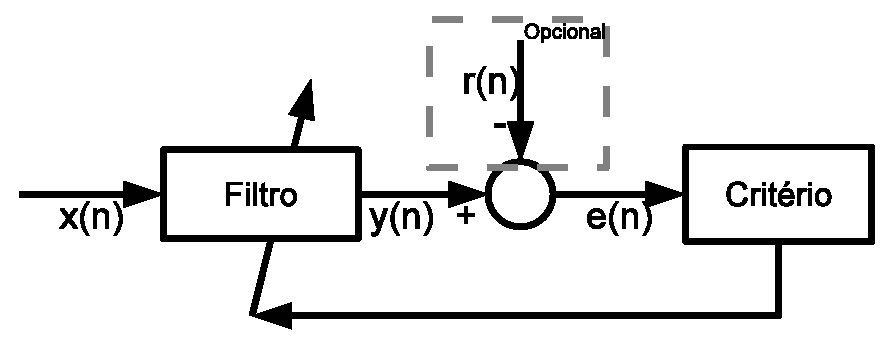
\includegraphics[width=.7\columnwidth]{cap1/filtering}
\caption{Esquema geral do problema de filtragem.}
\label{fig:filtering}
\end{figure}

Etiam id lobortis felis, dignissim commodo est. Nunc varius nulla et aliquam venenatis. Duis non neque ut tortor gravida viverra ut nec eros. Vestibulum et felis feugiat, lacinia ante et, tempus sem. Sed quis augue varius, sagittis lacus et, scelerisque felis. Morbi nec ligula ante. Maecenas vel sodales urna, vitae accumsan nisi. Maecenas lacinia adipiscing quam, eget elementum purus feugiat at. Fusce eget dictum sem. Maecenas ante ligula, tempus non mattis quis, ultrices vel elit. Nam porta est sit amet euismod pharetra. Integer vestibulum sem a sem volutpat, vitae adipiscing massa consequat. Aliquam iaculis mi in ultrices aliquet. Donec vitae semper sapien. Vivamus vel pretium enim.

Vestibulum ante ipsum primis in faucibus orci luctus et ultrices posuere cubilia Curae; Praesent porta ligula ipsum, ac lacinia leo malesuada ac. Morbi convallis in sapien at accumsan. Nunc sit amet tempus leo, adipiscing molestie leo. Sed ut arcu consequat lacus sagittis facilisis nec sit amet diam. Fusce a gravida dolor, eu sodales tellus. Ut porta nec velit at lacinia. Mauris felis arcu, faucibus eu porta vitae, luctus a nisl. Aenean tempus felis risus, sed vehicula ante fringilla quis. Integer eget purus a diam ultricies placerat. Donec consectetur vel urna id faucibus. In accumsan iaculis imperdiet. Nam venenatis enim quis nisl mattis, quis mattis neque tincidunt. Nullam sem enim, euismod ac nisi vel, viverra imperdiet augue.

\subsection{Subse\c{c}\~{a}o}
\label{sec:subsec01}

Maecenas condimentum nunc a tincidunt fermentum. Donec lobortis fermentum ante at hendrerit. Duis et gravida nisl. Nulla auctor dui sit amet mi tempor pretium eget fermentum nisi. Nam pharetra dolor eget ipsum consectetur porta. Ut ullamcorper enim a lacus dapibus, vel malesuada tellus posuere. Suspendisse sapien enim, cursus quis bibendum cursus, dapibus vel neque. Aliquam viverra, nulla in dictum dignissim, est nulla dapibus magna, id pretium tellus orci eget lacus. Interdum et malesuada fames ac ante ipsum primis in faucibus. Ut fermentum, erat at vulputate tempus, enim lorem elementum velit, eget tempus diam arcu at leo. Proin eu neque ac erat fermentum varius nec sit amet eros. Fusce arcu mi, consequat non nibh vel, tempus bibendum orci. Nulla vel nulla massa. Nullam sit amet velit aliquet, fringilla augue ac, congue nulla. Sed dignissim, magna eu posuere luctus, libero elit posuere sem, eu euismod ligula elit non sem.

Nullam lacinia ipsum vitae eros facilisis bibendum. Maecenas commodo neque dui, tristique porta sem ullamcorper ut. Vestibulum condimentum mauris eu egestas euismod. Nam vel ante congue libero accumsan mattis. Phasellus commodo euismod mi ac commodo. Proin quis volutpat massa. Curabitur non nunc sit amet augue placerat vulputate et fermentum arcu. In pellentesque lacinia tortor, quis vehicula arcu. Morbi lacinia vel ante ac tincidunt. Curabitur ac tincidunt eros.

Fusce id tellus nulla. Suspendisse aliquet sapien lacus, sit amet fermentum lacus pharetra a. Integer eu urna ut sem ultricies luctus in lacinia justo. Sed vel mattis orci, id egestas libero. Fusce ac libero aliquam neque faucibus cursus. Pellentesque pulvinar at nisl eget fermentum. Pellentesque quis interdum neque. Aenean vehicula euismod rutrum. Nulla luctus justo sit amet justo dignissim fermentum. Nunc eget ultrices dui, quis venenatis neque. Nullam volutpat nibh metus, sit amet convallis augue lacinia non. Maecenas eu est in nulla eleifend porttitor vel rutrum nisl.

Vestibulum erat purus, ultricies vehicula enim et, commodo posuere arcu. Pellentesque at orci metus. Aenean vestibulum mauris at nibh gravida, venenatis tempus augue sollicitudin. Curabitur nec justo odio. Cum sociis natoque penatibus et magnis dis parturient montes, nascetur ridiculus mus. Suspendisse varius ipsum at justo viverra mollis eu ac mauris. Nunc in facilisis erat. Ut aliquet tempus neque ac pretium. In viverra, risus imperdiet commodo commodo, orci tortor venenatis justo, sed ultricies nisi tortor at velit. Vivamus ultricies enim sit amet eleifend malesuada. Nullam at velit sem. Vivamus viverra tortor sed urna auctor interdum. 

\chapter{REVISÃO DA LITERATURA}
\label{cap:cap01}

Geralmente este capítulo é dedicado à revisão dos trabalhos que embasam o tema apresentado, assim como outros trabalhos já realizados no mesmo assunto. ”Revisão Bibliográfica” é apenas uma sugestão, porém o título deste capítulo pode ser diferente.

Sete normas da ABNT servem de base para a editoração de dissertações e teses. Algumas trazem uma apresentação do assunto, enquanto outras tratam de tópicos específicos: Referências (ABNT, 2002a), Citação em documentos (ABNT, 2002b), Trabalhos Acadêmicos (ABNT, 2011), Numeração progressiva das seções de um documento (ABNT, 2012a), Sumário (ABNT, 2012b), Resumo (ABNT, 2003) e Índice (ABNT, 2004). Em relação à formatação das figuras (ilustrações), este trabalho mantém a recomendação anterior da ABNT para Trabalhos Acadêmicos (ABNT, 2005).

Temos acesso as normas completas da ABNT em  www.bae.unicamp.br, link ‘normas técnicas’.


\section{Exemplo de Se\c{c}\~{a}o}
\label{sec:sec01}

Nunc malesuada posuere felis vel dapibus. Aliquam at fermentum lacus, vel malesuada elit. Duis varius nisi eget elit sagittis suscipit. Cras eu arcu at quam tristique facilisis eget vel ante. Quisque vitae libero lacinia, pellentesque tellus in, semper ligula. Aenean pharetra, elit vitae tristique pellentesque, justo erat luctus lectus, eget accumsan eros nisl vitae arcu. Proin consequat accumsan enim et porta. Aenean pharetra nulla risus, vitae ullamcorper ligula molestie in.

Integer ut elit lacus. Nullam id ullamcorper metus, et tincidunt mi. Donec blandit, sapien sit amet ultricies pharetra, turpis elit mollis risus, et pulvinar risus magna sed nunc. Sed eget risus ac risus consequat congue et ac nunc. Aenean a eros magna. Sed vel ante id ante venenatis feugiat. Sed et tortor dictum, pulvinar erat et, tempus felis. Donec pretium sagittis augue, non lacinia felis luctus a.

\begin{equation}
H(X) =-K\sum_{x\in\mathcal{X}} p_X(x)\log p_X(x),
\label{eq:shannonEntropy1}
\end{equation}

A equa\c{c}\~{a}o pode ser citada assim~\eqref{eq:shannonEntropy1}, e a se\c{c}\~{a}o assim~\ref{sec:sec01}

Aenean mauris sem, vulputate vitae vulputate vel, imperdiet volutpat erat. Nam malesuada pellentesque orci ac blandit. Maecenas pulvinar augue ac metus porttitor, eget tristique nunc vulputate. Sed nec mi mi. Curabitur ultrices facilisis consectetur. Cras vel urna porttitor, porta quam a, facilisis libero. Cras volutpat diam in tempor iaculis. Quisque rutrum vestibulum elit, sit amet gravida quam elementum ac. Fusce pretium hendrerit libero sed luctus. Phasellus sodales tristique purus non bibendum. Aenean faucibus pulvinar ligula, ut aliquam eros varius adipiscing. Ut a ipsum tempor, placerat quam non, imperdiet mi.

%\begin{figure}[htb]
%\centering
%	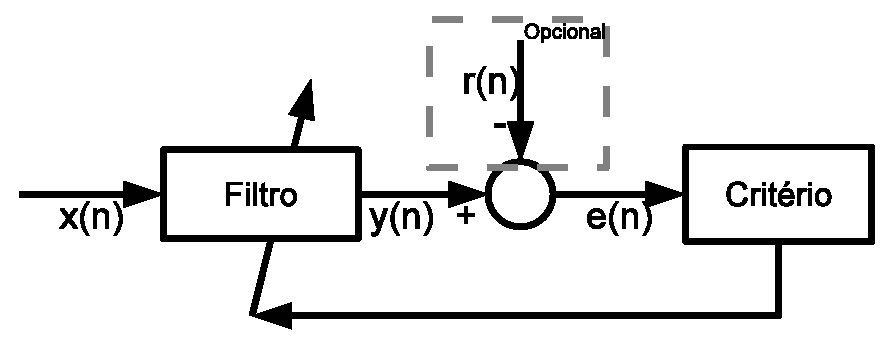
\includegraphics[width=.7\columnwidth]{cap1/filtering}
%\caption{Esquema geral do problema de filtragem.}
%\label{fig:filtering}
%\end{figure}

Etiam id lobortis felis, dignissim commodo est. Nunc varius nulla et aliquam venenatis. Duis non neque ut tortor gravida viverra ut nec eros. Vestibulum et felis feugiat, lacinia ante et, tempus sem. Sed quis augue varius, sagittis lacus et, scelerisque felis. Morbi nec ligula ante. Maecenas vel sodales urna, vitae accumsan nisi. Maecenas lacinia adipiscing quam, eget elementum purus feugiat at. Fusce eget dictum sem. Maecenas ante ligula, tempus non mattis quis, ultrices vel elit. Nam porta est sit amet euismod pharetra. Integer vestibulum sem a sem volutpat, vitae adipiscing massa consequat. Aliquam iaculis mi in ultrices aliquet. Donec vitae semper sapien. Vivamus vel pretium enim.

Vestibulum ante ipsum primis in faucibus orci luctus et ultrices posuere cubilia Curae; Praesent porta ligula ipsum, ac lacinia leo malesuada ac. Morbi convallis in sapien at accumsan. Nunc sit amet tempus leo, adipiscing molestie leo. Sed ut arcu consequat lacus sagittis facilisis nec sit amet diam. Fusce a gravida dolor, eu sodales tellus. Ut porta nec velit at lacinia. Mauris felis arcu, faucibus eu porta vitae, luctus a nisl. Aenean tempus felis risus, sed vehicula ante fringilla quis. Integer eget purus a diam ultricies placerat. Donec consectetur vel urna id faucibus. In accumsan iaculis imperdiet. Nam venenatis enim quis nisl mattis, quis mattis neque tincidunt. Nullam sem enim, euismod ac nisi vel, viverra imperdiet augue.

\subsection{Subse\c{c}\~{a}o}
\label{sec:subsec01}

Maecenas condimentum nunc a tincidunt fermentum. Donec lobortis fermentum ante at hendrerit. Duis et gravida nisl. Nulla auctor dui sit amet mi tempor pretium eget fermentum nisi. Nam pharetra dolor eget ipsum consectetur porta. Ut ullamcorper enim a lacus dapibus, vel malesuada tellus posuere. Suspendisse sapien enim, cursus quis bibendum cursus, dapibus vel neque. Aliquam viverra, nulla in dictum dignissim, est nulla dapibus magna, id pretium tellus orci eget lacus. Interdum et malesuada fames ac ante ipsum primis in faucibus. Ut fermentum, erat at vulputate tempus, enim lorem elementum velit, eget tempus diam arcu at leo. Proin eu neque ac erat fermentum varius nec sit amet eros. Fusce arcu mi, consequat non nibh vel, tempus bibendum orci. Nulla vel nulla massa. Nullam sit amet velit aliquet, fringilla augue ac, congue nulla. Sed dignissim, magna eu posuere luctus, libero elit posuere sem, eu euismod ligula elit non sem.

Nullam lacinia ipsum vitae eros facilisis bibendum. Maecenas commodo neque dui, tristique porta sem ullamcorper ut. Vestibulum condimentum mauris eu egestas euismod. Nam vel ante congue libero accumsan mattis. Phasellus commodo euismod mi ac commodo. Proin quis volutpat massa. Curabitur non nunc sit amet augue placerat vulputate et fermentum arcu. In pellentesque lacinia tortor, quis vehicula arcu. Morbi lacinia vel ante ac tincidunt. Curabitur ac tincidunt eros.

Fusce id tellus nulla. Suspendisse aliquet sapien lacus, sit amet fermentum lacus pharetra a. Integer eu urna ut sem ultricies luctus in lacinia justo. Sed vel mattis orci, id egestas libero. Fusce ac libero aliquam neque faucibus cursus. Pellentesque pulvinar at nisl eget fermentum. Pellentesque quis interdum neque. Aenean vehicula euismod rutrum. Nulla luctus justo sit amet justo dignissim fermentum. Nunc eget ultrices dui, quis venenatis neque. Nullam volutpat nibh metus, sit amet convallis augue lacinia non. Maecenas eu est in nulla eleifend porttitor vel rutrum nisl.

Vestibulum erat purus, ultricies vehicula enim et, commodo posuere arcu. Pellentesque at orci metus. Aenean vestibulum mauris at nibh gravida, venenatis tempus augue sollicitudin. Curabitur nec justo odio. Cum sociis natoque penatibus et magnis dis parturient montes, nascetur ridiculus mus. Suspendisse varius ipsum at justo viverra mollis eu ac mauris. Nunc in facilisis erat. Ut aliquet tempus neque ac pretium. In viverra, risus imperdiet commodo commodo, orci tortor venenatis justo, sed ultricies nisi tortor at velit. Vivamus ultricies enim sit amet eleifend malesuada. Nullam at velit sem. Vivamus viverra tortor sed urna auctor interdum.

%\resetlinenumber
%\chapter{METODOLOGIA}
\label{cap:cap02}

Neste t\'{o}pico deve ser descrito minuciosamente toda a\c{c}\~{a}o desenvolvida na aplica\c{c}\~{a}o do m\'{e}todo cient\'{\i}fico utilizado, bem como o tipo de pesquisa, instrumentos, tempo de execu\c{c}\~{a}o.
Al\'{e}m dos outros tipos de pesquisa que o trabalho pode conter, a pesquisa bibliogr\'{a}fica \'{e} uma etapa fundamental pois fornece o embasamento do trabalho. Consiste no levantamento, sele\c{c}\~{a}o, fichamento de informa\c{c}\~{o}es relacionadas \`{a} pesquisa bibliogr\'{a}fica como livros, revistas, jornais, teses, disserta\c{c}\~{o}es, anais, etc e descreve as bases de dados pesquisadas, os assuntos/ descritores/metadados, limitadores/filtros, etc. Tal etapa pode ser melhor aproveitada solicitando ajuda \`{a} Biblioteca.
\cite{Cover2006,Feynman1998,Haykin2001}

\section{Exemplo de Se\c{c}\~{a}o}
\label{sec:sec02}

Nunc malesuada posuere felis vel dapibus. Aliquam at fermentum lacus, vel malesuada elit. Duis varius nisi eget elit sagittis suscipit. Cras eu arcu at quam tristique facilisis eget vel ante. Quisque vitae libero lacinia, pellentesque tellus in, semper ligula. Aenean pharetra, elit vitae tristique pellentesque, justo erat luctus lectus, eget accumsan eros nisl vitae arcu. Proin consequat accumsan enim et porta. Aenean pharetra nulla risus, vitae ullamcorper ligula molestie in.

Integer ut elit lacus. Nullam id ullamcorper metus, et tincidunt mi. Donec blandit, sapien sit amet ultricies pharetra, turpis elit mollis risus, et pulvinar risus magna sed nunc. Sed eget risus ac risus consequat congue et ac nunc. Aenean a eros magna. Sed vel ante id ante venenatis feugiat. Sed et tortor dictum, pulvinar erat et, tempus felis. Donec pretium sagittis augue, non lacinia felis luctus a.

\begin{equation}
H(X) =-K\sum_{x\in\mathcal{X}} p_X(x)\log p_X(x),
\label{eq:shannonEntropy}
\end{equation}

A equa\c{c}\~{a}o pode ser citada assim~\eqref{eq:shannonEntropy}, e a se\c{c}\~{a}o assim~\ref{sec:sec02}

Aenean mauris sem, vulputate vitae vulputate vel, imperdiet volutpat erat. Nam malesuada pellentesque orci ac blandit. Maecenas pulvinar augue ac metus porttitor, eget tristique nunc vulputate. Sed nec mi mi. Curabitur ultrices facilisis consectetur. Cras vel urna porttitor, porta quam a, facilisis libero. Cras volutpat diam in tempor iaculis. Quisque rutrum vestibulum elit, sit amet gravida quam elementum ac. Fusce pretium hendrerit libero sed luctus. Phasellus sodales tristique purus non bibendum. Aenean faucibus pulvinar ligula, ut aliquam eros varius adipiscing. Ut a ipsum tempor, placerat quam non, imperdiet mi.

Etiam id lobortis felis, dignissim commodo est. Nunc varius nulla et aliquam venenatis. Duis non neque ut tortor gravida viverra ut nec eros. Vestibulum et felis feugiat, lacinia ante et, tempus sem. Sed quis augue varius, sagittis lacus et, scelerisque felis. Morbi nec ligula ante. Maecenas vel sodales urna, vitae accumsan nisi. Maecenas lacinia adipiscing quam, eget elementum purus feugiat at. Fusce eget dictum sem. Maecenas ante ligula, tempus non mattis quis, ultrices vel elit. Nam porta est sit amet euismod pharetra. Integer vestibulum sem a sem volutpat, vitae adipiscing massa consequat. Aliquam iaculis mi in ultrices aliquet. Donec vitae semper sapien. Vivamus vel pretium enim.

Vestibulum ante ipsum primis in faucibus orci luctus et ultrices posuere cubilia Curae; Praesent porta ligula ipsum, ac lacinia leo malesuada ac. Morbi convallis in sapien at accumsan. Nunc sit amet tempus leo, adipiscing molestie leo. Sed ut arcu consequat lacus sagittis facilisis nec sit amet diam. Fusce a gravida dolor, eu sodales tellus. Ut porta nec velit at lacinia. Mauris felis arcu, faucibus eu porta vitae, luctus a nisl. Aenean tempus felis risus, sed vehicula ante fringilla quis. Integer eget purus a diam ultricies placerat. Donec consectetur vel urna id faucibus. In accumsan iaculis imperdiet. Nam venenatis enim quis nisl mattis, quis mattis neque tincidunt. Nullam sem enim, euismod ac nisi vel, viverra imperdiet augue.

\subsection{Subse\c{c}\~{a}o}
\label{sec:subsec02}

Maecenas condimentum nunc a tincidunt fermentum. Donec lobortis fermentum ante at hendrerit. Duis et gravida nisl. Nulla auctor dui sit amet mi tempor pretium eget fermentum nisi. Nam pharetra dolor eget ipsum consectetur porta. Ut ullamcorper enim a lacus dapibus, vel malesuada tellus posuere. Suspendisse sapien enim, cursus quis bibendum cursus, dapibus vel neque. Aliquam viverra, nulla in dictum dignissim, est nulla dapibus magna, id pretium tellus orci eget lacus. Interdum et malesuada fames ac ante ipsum primis in faucibus. Ut fermentum, erat at vulputate tempus, enim lorem elementum velit, eget tempus diam arcu at leo. Proin eu neque ac erat fermentum varius nec sit amet eros. Fusce arcu mi, consequat non nibh vel, tempus bibendum orci. Nulla vel nulla massa. Nullam sit amet velit aliquet, fringilla augue ac, congue nulla. Sed dignissim, magna eu posuere luctus, libero elit posuere sem, eu euismod ligula elit non sem.

\subsection{Exemplo de Imagens}

As Figuras \ref{fig:figura_1_exemplo}, \ref{fig:figura_2_exemplo} e \ref{fig:figura_3_exemplo} ilustram como posicionar tr\^{e}s imagens em duas colunas. As Figuras \ref{fig:figura_4_exemplo}, \ref{fig:figura_5_exemplo}, \ref{fig:figura_6_exemplo}, \ref{fig:figura_7_exemplo} ilustram como posicionar 4 imagens em duas colunas e duas linhas, cada imagem com sua respectiva legenda, e como referenciar cada imagem individualmente. H\'{a} op\c{c}\~{a}o tamb\'{e}m de referenciar a imagem \ref{fig:exemplo_imagens} como um todo.

\begin{figure}[ht!]
	\centering
	\begin{minipage}[b]{.45\textwidth}
		\centering
        \subfloat[Figura 1.\label{fig:figura_1_exemplo}]{\includegraphics[width=\textwidth]{./Figuras/feec.eps}}		
	\end{minipage}\qquad
	\begin{minipage}[b]{.45\textwidth}
		\centering
		\subfloat[Figura 2.\label{fig:figura_2_exemplo}]{
\includegraphics[scale=0.2]{./Figuras/unicamp2.eps}}
		\vspace{2ex}		
		
        \subfloat[Figura 3.\label{fig:figura_3_exemplo}]{
\includegraphics[scale=1]{./Figuras/unicamp4.png}}% Note como a qualidade da imagem eps no pdf \'{e} superior visualmente
	\end{minipage}
	\caption{Exemplo de imagens.\label{fig:figuras_exemplos}}
\end{figure}

\begin{figure}
    \centering
    \subfloat[Legenda da Figura da Esquerda.\label{fig:figura_1_exemplo1}]{\includegraphics[width=0.40\textwidth]{./Figuras/unicamp1.eps}}
    \hspace{0.5cm}
    \subfloat[Legenda da Figura da Direita.\label{fig:figura_2_exemplo1}]{
\includegraphics[width=0.40\textwidth]{./Figuras/unicamp2.eps}}
    \caption{Figura com duas subfiguras utilizando o pacote \textit{\textbackslash subfig}}\label{fig:exemplo_2_imagens_subfloat}
\end{figure}

\begin{figure}[ht]
    \centering
    \label{ fig8}
    \begin{minipage}[b]{0.45\textwidth}
        \centering
        \subfloat[Legenda da Figura da Esquerda Superior.\label{fig:figura_4_exemplo}]{\includegraphics[width=0.9\textwidth]{./Figuras/unicamp1.eps}}
    \end{minipage}%%
    \begin{minipage}[b]{0.45\textwidth}
        \centering
        \subfloat[Legenda da Figura da Direita Superior.\label{fig:figura_5_exemplo}]{
\includegraphics[width=0.9\textwidth]{./Figuras/unicamp2.eps}}
    \end{minipage}
    \vskip\baselineskip
    \begin{minipage}[b]{0.45\textwidth}
        \centering
        \subfloat[Legenda da Figura da Esquerda Inferior.\label{fig:figura_6_exemplo}]{
\includegraphics[width=0.9\textwidth]{./Figuras/unicamp3.eps}}
    \end{minipage}%%
    \begin{minipage}[b]{0.45\textwidth}
        \centering
        \subfloat[Legenda da Figura da Direita Inferior.\label{fig:figura_7_exemplo}]{
\includegraphics[scale=1.3]{./Figuras/unicamp4.eps}}
    \end{minipage}
    \caption{Figura com quatro subfiguras utilizando o pacote \textit{\textbackslash subfig} e \textit{minipage}}\label{fig:exemplo_imagens}
\end{figure}



%\begin{figure}
%  \centering
%
%    \centering
%    \subcaptionbox{First top left}
%      {\includegraphics[width=\linewidth,height=50pt]{./Figuras/unicamp1.eps}}
%
%    \subcaptionbox{Second top left}
%      {\includegraphics[width=\linewidth,height=50pt]{./Figuras/unicamp1.eps}}
%
%    \subcaptionbox{Third top left}
%      {\includegraphics[width=\linewidth,height=50pt]{./Figuras/unicamp1.eps}}
%\end{figure}

%\begin{figure}[H]
%	\centering
%	\begin{subfigure}[t]{0.45\textwidth}
%		\centering
%		\includegraphics[width=\textwidth]{./Figuras/unicamp1.eps}
%		\caption{Figura 4.}
%		\label{fig:figura_4_exemplo}
%	\end{subfigure}%
%	~
%	\begin{subfigure}[t]{0.45\textwidth}
%		\centering
%		
\includegraphics[width=\textwidth]{./Figuras/unicamp2.eps}
%		\caption{Figura 5.}
%		\label{fig:figura_5_exemplo}
%	\end{subfigure}
%	
%	\begin{subfigure}[t]{0.45\textwidth}
%		\centering
%		
\includegraphics[width=\textwidth]{./Figuras/unicamp3.eps}
%		\caption{Figura 6.}
%		\label{fig:figura_6_exemplo}
%	\end{subfigure}%
%	~
%	\begin{subfigure}[t]{0.45\textwidth}
%		\centering
%		
\includegraphics[scale=1]{./Figuras/unicamp4.eps}
%		\caption{Figura 7.}
%		\label{fig:figura_7_exemplo}
%	\end{subfigure}
%	\caption{Exemplo de imagens.}
%	\label{fig:exemplo_imagens}
%\end{figure}


\chapter{METODOLOGIA}
\label{cap:cap02}

Neste t\'{o}pico deve ser descrito minuciosamente toda a\c{c}\~{a}o desenvolvida na aplica\c{c}\~{a}o do m\'{e}todo cient\'{\i}fico utilizado, bem como o tipo de pesquisa, instrumentos, tempo de execu\c{c}\~{a}o.
Al\'{e}m dos outros tipos de pesquisa que o trabalho pode conter, a pesquisa bibliogr\'{a}fica \'{e} uma etapa fundamental pois fornece o embasamento do trabalho. Consiste no levantamento, sele\c{c}\~{a}o, fichamento de informa\c{c}\~{o}es relacionadas \`{a} pesquisa bibliogr\'{a}fica como livros, revistas, jornais, teses, disserta\c{c}\~{o}es, anais, etc e descreve as bases de dados pesquisadas, os assuntos/ descritores/metadados, limitadores/filtros, etc. Tal etapa pode ser melhor aproveitada solicitando ajuda \`{a} Biblioteca.
\cite{Cover2006,Feynman1998,Haykin2001}

\section{Exemplo de Se\c{c}\~{a}o}
\label{sec:sec02}

Nunc malesuada posuere felis vel dapibus. Aliquam at fermentum lacus, vel malesuada elit. Duis varius nisi eget elit sagittis suscipit. Cras eu arcu at quam tristique facilisis eget vel ante. Quisque vitae libero lacinia, pellentesque tellus in, semper ligula. Aenean pharetra, elit vitae tristique pellentesque, justo erat luctus lectus, eget accumsan eros nisl vitae arcu. Proin consequat accumsan enim et porta. Aenean pharetra nulla risus, vitae ullamcorper ligula molestie in.

Integer ut elit lacus. Nullam id ullamcorper metus, et tincidunt mi. Donec blandit, sapien sit amet ultricies pharetra, turpis elit mollis risus, et pulvinar risus magna sed nunc. Sed eget risus ac risus consequat congue et ac nunc. Aenean a eros magna. Sed vel ante id ante venenatis feugiat. Sed et tortor dictum, pulvinar erat et, tempus felis. Donec pretium sagittis augue, non lacinia felis luctus a.

\begin{equation}
H(X) =-K\sum_{x\in\mathcal{X}} p_X(x)\log p_X(x),
\label{eq:shannonEntropy}
\end{equation}

A equa\c{c}\~{a}o pode ser citada assim~\eqref{eq:shannonEntropy}, e a se\c{c}\~{a}o assim~\ref{sec:sec02}

Aenean mauris sem, vulputate vitae vulputate vel, imperdiet volutpat erat. Nam malesuada pellentesque orci ac blandit. Maecenas pulvinar augue ac metus porttitor, eget tristique nunc vulputate. Sed nec mi mi. Curabitur ultrices facilisis consectetur. Cras vel urna porttitor, porta quam a, facilisis libero. Cras volutpat diam in tempor iaculis. Quisque rutrum vestibulum elit, sit amet gravida quam elementum ac. Fusce pretium hendrerit libero sed luctus. Phasellus sodales tristique purus non bibendum. Aenean faucibus pulvinar ligula, ut aliquam eros varius adipiscing. Ut a ipsum tempor, placerat quam non, imperdiet mi.

Etiam id lobortis felis, dignissim commodo est. Nunc varius nulla et aliquam venenatis. Duis non neque ut tortor gravida viverra ut nec eros. Vestibulum et felis feugiat, lacinia ante et, tempus sem. Sed quis augue varius, sagittis lacus et, scelerisque felis. Morbi nec ligula ante. Maecenas vel sodales urna, vitae accumsan nisi. Maecenas lacinia adipiscing quam, eget elementum purus feugiat at. Fusce eget dictum sem. Maecenas ante ligula, tempus non mattis quis, ultrices vel elit. Nam porta est sit amet euismod pharetra. Integer vestibulum sem a sem volutpat, vitae adipiscing massa consequat. Aliquam iaculis mi in ultrices aliquet. Donec vitae semper sapien. Vivamus vel pretium enim.

Vestibulum ante ipsum primis in faucibus orci luctus et ultrices posuere cubilia Curae; Praesent porta ligula ipsum, ac lacinia leo malesuada ac. Morbi convallis in sapien at accumsan. Nunc sit amet tempus leo, adipiscing molestie leo. Sed ut arcu consequat lacus sagittis facilisis nec sit amet diam. Fusce a gravida dolor, eu sodales tellus. Ut porta nec velit at lacinia. Mauris felis arcu, faucibus eu porta vitae, luctus a nisl. Aenean tempus felis risus, sed vehicula ante fringilla quis. Integer eget purus a diam ultricies placerat. Donec consectetur vel urna id faucibus. In accumsan iaculis imperdiet. Nam venenatis enim quis nisl mattis, quis mattis neque tincidunt. Nullam sem enim, euismod ac nisi vel, viverra imperdiet augue.

\subsection{Subse\c{c}\~{a}o}
\label{sec:subsec02}

Maecenas condimentum nunc a tincidunt fermentum. Donec lobortis fermentum ante at hendrerit. Duis et gravida nisl. Nulla auctor dui sit amet mi tempor pretium eget fermentum nisi. Nam pharetra dolor eget ipsum consectetur porta. Ut ullamcorper enim a lacus dapibus, vel malesuada tellus posuere. Suspendisse sapien enim, cursus quis bibendum cursus, dapibus vel neque. Aliquam viverra, nulla in dictum dignissim, est nulla dapibus magna, id pretium tellus orci eget lacus. Interdum et malesuada fames ac ante ipsum primis in faucibus. Ut fermentum, erat at vulputate tempus, enim lorem elementum velit, eget tempus diam arcu at leo. Proin eu neque ac erat fermentum varius nec sit amet eros. Fusce arcu mi, consequat non nibh vel, tempus bibendum orci. Nulla vel nulla massa. Nullam sit amet velit aliquet, fringilla augue ac, congue nulla. Sed dignissim, magna eu posuere luctus, libero elit posuere sem, eu euismod ligula elit non sem.

\subsection{Exemplo de Imagens}

As Figuras \ref{fig:figura_1_exemplo}, \ref{fig:figura_2_exemplo} e \ref{fig:figura_3_exemplo} ilustram como posicionar tr\^{e}s imagens em duas colunas. As Figuras \ref{fig:figura_4_exemplo}, \ref{fig:figura_5_exemplo}, \ref{fig:figura_6_exemplo}, \ref{fig:figura_7_exemplo} ilustram como posicionar 4 imagens em duas colunas e duas linhas, cada imagem com sua respectiva legenda, e como referenciar cada imagem individualmente. H\'{a} op\c{c}\~{a}o tamb\'{e}m de referenciar a imagem \ref{fig:exemplo_imagens} como um todo.

\begin{figure}[ht!]
	\centering
	\begin{minipage}[b]{.45\textwidth}
		\centering
        \subfloat[Figura 1.\label{fig:figura_1_exemplo}]{\includegraphics[width=\textwidth]{./figures/feec.eps}}
	\end{minipage}\qquad
	\begin{minipage}[b]{.45\textwidth}
		\centering
		\subfloat[Figura 2.\label{fig:figura_2_exemplo}]{
\includegraphics[scale=0.2]{./figures/unicamp2.eps}}
		\vspace{2ex}

        \subfloat[Figura 3.\label{fig:figura_3_exemplo}]{
\includegraphics[scale=1]{./figures/unicamp4.png}}% Note como a qualidade da imagem eps no pdf \'{e} superior visualmente
	\end{minipage}
	\caption{Exemplo de imagens.\label{fig:figuras_exemplos}}
\end{figure}

\begin{figure}
    \centering
    \subfloat[Legenda da Figura da Esquerda.\label{fig:figura_1_exemplo1}]{\includegraphics[width=0.40\textwidth]{./figures/unicamp1.eps}}
    \hspace{0.5cm}
    \subfloat[Legenda da Figura da Direita.\label{fig:figura_2_exemplo1}]{
\includegraphics[width=0.40\textwidth]{./figures/unicamp2.eps}}
    \caption{Figura com duas subfiguras utilizando o pacote \textit{\textbackslash subfig}}\label{fig:exemplo_2_imagens_subfloat}
\end{figure}

\begin{figure}[ht]
    \centering
    \label{ fig8}
    \begin{minipage}[b]{0.45\textwidth}
        \centering
        \subfloat[Legenda da Figura da Esquerda Superior.\label{fig:figura_4_exemplo}]{\includegraphics[width=0.9\textwidth]{./figures/unicamp1.eps}}
    \end{minipage}%%
    \begin{minipage}[b]{0.45\textwidth}
        \centering
        \subfloat[Legenda da Figura da Direita Superior.\label{fig:figura_5_exemplo}]{
\includegraphics[width=0.9\textwidth]{./figures/unicamp2.eps}}
    \end{minipage}
    \vskip\baselineskip
    \begin{minipage}[b]{0.45\textwidth}
        \centering
        \subfloat[Legenda da Figura da Esquerda Inferior.\label{fig:figura_6_exemplo}]{
\includegraphics[width=0.9\textwidth]{./figures/unicamp3.eps}}
    \end{minipage}%%
    \begin{minipage}[b]{0.45\textwidth}
        \centering
        \subfloat[Legenda da Figura da Direita Inferior.\label{fig:figura_7_exemplo}]{
\includegraphics[scale=1.3]{./figures/unicamp4.eps}}
    \end{minipage}
    \caption{Figura com quatro subfiguras utilizando o pacote \textit{\textbackslash subfig} e \textit{minipage}}\label{fig:exemplo_imagens}
\end{figure}



%\begin{figure}
%  \centering
%
%    \centering
%    \subcaptionbox{First top left}
%      {\includegraphics[width=\linewidth,height=50pt]{./figures/unicamp1.eps}}
%
%    \subcaptionbox{Second top left}
%      {\includegraphics[width=\linewidth,height=50pt]{./figures/unicamp1.eps}}
%
%    \subcaptionbox{Third top left}
%      {\includegraphics[width=\linewidth,height=50pt]{./figures/unicamp1.eps}}
%\end{figure}

%\begin{figure}[H]
%	\centering
%	\begin{subfigure}[t]{0.45\textwidth}
%		\centering
%		\includegraphics[width=\textwidth]{./figures/unicamp1.eps}
%		\caption{Figura 4.}
%		\label{fig:figura_4_exemplo}
%	\end{subfigure}%
%	~
%	\begin{subfigure}[t]{0.45\textwidth}
%		\centering
%		
\includegraphics[width=\textwidth]{./figures/unicamp2.eps}
%		\caption{Figura 5.}
%		\label{fig:figura_5_exemplo}
%	\end{subfigure}
%
%	\begin{subfigure}[t]{0.45\textwidth}
%		\centering
%		
\includegraphics[width=\textwidth]{./figures/unicamp3.eps}
%		\caption{Figura 6.}
%		\label{fig:figura_6_exemplo}
%	\end{subfigure}%
%	~
%	\begin{subfigure}[t]{0.45\textwidth}
%		\centering
%		
\includegraphics[scale=1]{./figures/unicamp4.eps}
%		\caption{Figura 7.}
%		\label{fig:figura_7_exemplo}
%	\end{subfigure}
%	\caption{Exemplo de imagens.}
%	\label{fig:exemplo_imagens}
%\end{figure}

%\resetlinenumber
%\chapter{AN\'{A}LISE DOS DADOS}

A An\'{a}lise e interpreta\c{c}\~{a}o dos dados \'{e} o tratamento dos dados, a articula\c{c}\~{a}o com teoria e m\'{e}todos espec\'{\i}ficos utilizados.\cite{Cover2006}

\resetlinenumber
\chapter{RESULTADOS E DISCUSS\~{O}ES }

\'{E} a apresenta\c{c}\~{a}o dos principais resultados advindos do t\'{o}pico ‘an\'{a}lise dos dados’.\cite{Feynman1998}


\chapter{ANÁLISE DOS DADOS}

A An\'{a}lise e interpreta\c{c}\~{a}o dos dados \'{e} o tratamento dos dados, a articula\c{c}\~{a}o com teoria e m\'{e}todos espec\'{\i}ficos utilizados.\cite{Cover2006}

\resetlinenumber
\chapter{RESULTADOS E DISCUSS\~{O}ES }

\'{E} a apresenta\c{c}\~{a}o dos principais resultados advindos do t\'{o}pico ‘an\'{a}lise dos dados’.\cite{Feynman1998}

% ----------------------------------------------------------
% Finaliza a parte no bookmark do PDF
% para que se inicie o bookmark na raiz
% e adiciona espa\c{c}o de parte no Sum\'{a}rio
% ----------------------------------------------------------
\phantompart

% ---
% Conclus\~{a}o
% ---
\resetlinenumber
\chapter{Conclus\~{a}o}
% ---

\lipsum[31-33]


\nolinenumbers  %Não numerar referências


% ----------------------------------------------------------
% ELEMENTOS P\'{O}S-TEXTUAIS
% ----------------------------------------------------------
\postextual
% ----------------------------------------------------------

% ----------------------------------------------------------
% Refer\^{e}ncias bibliogr\'{a}ficas
% ----------------------------------------------------------
\bibliography{tese}

% ----------------------------------------------------------
% Gloss\'{a}rio
% ----------------------------------------------------------
%
% Consulte o manual da classe abntex2 para orienta\c{c}\~{o}es sobre o gloss\'{a}rio.
%
%\glossary

% ----------------------------------------------------------
% Ap\^{e}ndices
% ----------------------------------------------------------

% ---
% Inicia os ap\^{e}ndices
% ---
\begin{apendicesenv}

% Imprime uma p\'{a}gina indicando o in\'{\i}cio dos ap\^{e}ndices
\partapendices

% ----------------------------------------------------------
\chapter{Quisque libero justo}
% ----------------------------------------------------------

\lipsum[50]

% ----------------------------------------------------------
\chapter{Nullam elementum urna vel imperdiet sodales elit ipsum pharetra ligula
ac pretium ante justo a nulla curabitur tristique arcu eu metus}
% ----------------------------------------------------------
\lipsum[55-57]

\end{apendicesenv}
% ---


% ----------------------------------------------------------
% Anexos
% ----------------------------------------------------------

% ---
% Inicia os anexos
% ---
\begin{anexosenv}

% Imprime uma p\'{a}gina indicando o in\'{\i}cio dos anexos
\partanexos

% ---
\chapter{Morbi ultrices rutrum lorem.}
% ---
\lipsum[30]

% ---
\chapter{Cras non urna sed feugiat cum sociis natoque penatibus et magnis dis
parturient montes nascetur ridiculus mus}
% ---

\lipsum[31]

% ---
\chapter{Fusce facilisis lacinia dui}
% ---

\lipsum[32]

\end{anexosenv}

%---------------------------------------------------------------------
% INDICE REMISSIVO
%---------------------------------------------------------------------
\phantompart
\printindex
%---------------------------------------------------------------------

\end{document}
